\chapter{Versuchsaufbau}
    \section{Reihenschaltung und Parallelschaltung}
        In den Aufgaben wurde vorgegeben das wir eine Spannungsquelle mit einem Sinussignal $U_{pri}=230\,V$ und einer Frequenze von $50\,Hz$ verwenden sollen. 
        Die Spannung ist als Effektivwert gegeben, die man erst noch umrechnen muss. Das wie folgt abläuft. 
        \begin{gather}
            U_{eff}=\frac{\widehat{u}}{\sqrt{2}}\\
            \widehat{u} =U_{eff}\sqrt{2}\Rightarrow \widehat{u} =230\,V\sqrt{2}=325,269\,V
        \end{gather}
        In den Weiteren Aufgaben wird mit $325\,V$  gearbeitet.\par

        Im Versuch wird der Transformator RSO826007 von der Firma SedlbauerAG verwendet. Die Sekundärsüulen des Transformators werden sowohl on Reihe als auch Parallel (siehe Abb.~\ref{fig:reihenschaltung} und Abb.~\ref{fig:parallelschaltung} ) mit einem Wiederstand geschaltet. 
        Die verkabelung des Transformators wurden dem Datenblatt entnommen (\href{www.sedlbauer.de/media/ringkerntrafo_datenblatt_825007.pdf}{www.sedlbauer.de/media/ringkerntrafo\_datenblatt\_825007.pdf}).

        \begin{figure}[ht!]
            \begin{minipage}[c]{0.5\textwidth}
                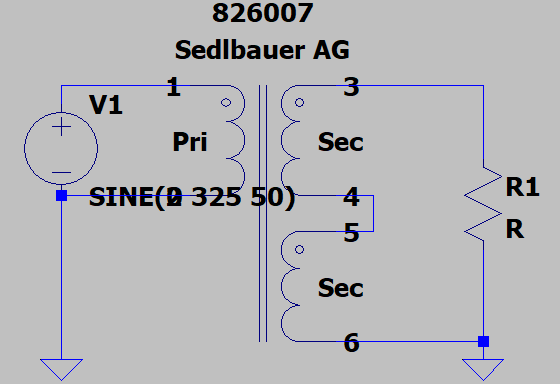
\includegraphics[width=.9\linewidth]{Bilder/transformator_reihe.PNG}
                \caption{Schaltbild der Reihenschaltung}
                \label{fig:reihenschaltung}
            \end{minipage}
            \begin{minipage}[c]{0.5\textwidth}
                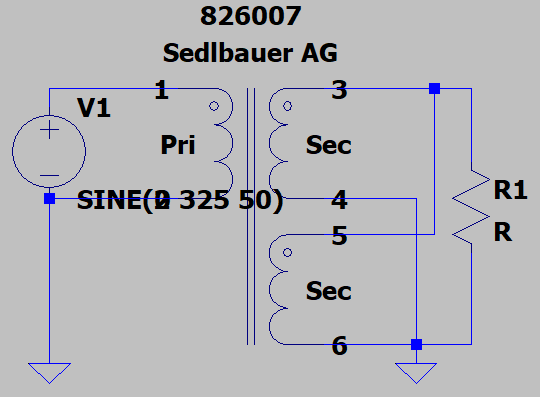
\includegraphics[width=.9\linewidth]{Bilder/transformator_parallel.png}
                \caption{Schaltbild der Parallelschaltung}
                \label{fig:parallelschaltung}
            \end{minipage}
        \end{figure}
    \newpage
    \section{Schaltbild mit einem Brückengleichrichter und Glättungskondensator}
        In der zweiten Teilaufgabe wird ein Brückengleichrichter mit Glättungskondensator an den Transformator angeschloßen \fref{fig:gleichrichter}.
        In der Schaltung sind Dioden vom Type \textit{MURS320}, für den Brückengleichrichter, eingebaut. Desweiteren ist für die Realisierung eines Glättungskondensator ein Kondensator vom Typ \textit{UPL1C102MPH} eingebaut worden. Es ist zu beachten das der Lastwiderstand an dem Schaltung entfällt. Dieser wird durch einen Laststrom ($100 \, mA$) ersetzt.


        \begin{figure}[ht!]
            \centering
            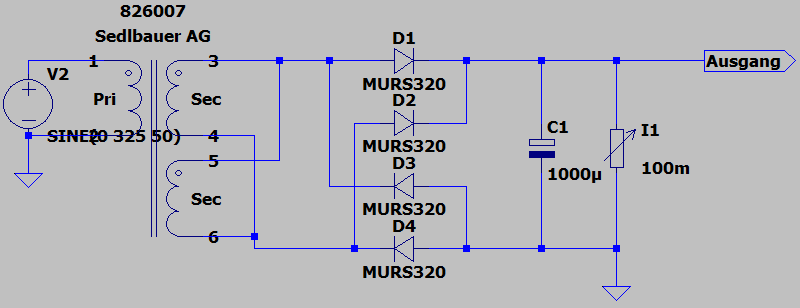
\includegraphics[width=.9\textwidth]{Bilder/gleichrichter.PNG}
            \caption{Schaltbild mit einem Brückengleichrichter und Glättungskondensator}
            \label{fig:gleichrichter}
        \end{figure}